% *********************************************************************
% © 2024–2026 Jeremy Sylvestre
%
% Permission is granted to copy, distribute and/or modify this document
% under the terms of the GNU Free Documentation License, Version 1.3 or
% any later version published by the Free Software Foundation; with no
% Invariant Sections, no Front-Cover Texts, and no Back-Cover Texts. A
% copy of the license is included in the appendix entitled “GNU Free
% Documentation License” that appears in the output document of this
% PreTeXt source code. All trademarks™ are the registered® marks of
% their respective owners.
%
% *********************************************************************

\newcommand*{\xmin}{-0.333}
\newcommand*{\xmax}{6.05}
\newcommand*{\ymin}{-0.1}
\newcommand*{\ymax}{1.5}

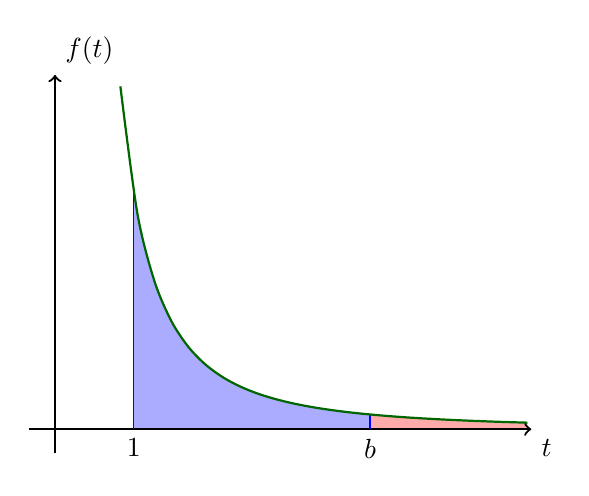
\begin{tikzpicture}[yscale=3]

	\fill[blue,opacity=0.33] plot[domain=1:4,smooth] (\x,{1 / (\x * \x)}) -- (4,0) -- (1,0) -- (1,1);

	\fill[red,opacity=0.33] plot[domain=4:6,smooth] (\x,{1 / (\x * \x)}) -- (6,0) -- (4,0) -- (4,0.0625);

	% axes
	\draw[->,thick] (\xmin,0) -- (\xmax,0) node[below right] {$t$};
	\draw[->,thick] (0,\ymin) -- (0,\ymax) node[above right] {$f(t)$};

	\draw[blue,thin] (1,1) -- (1,0) node[black,below] {$1$};
	\draw[blue,thin] (4,0.0625) -- (4,0) node[black,below] {$b$};

	\draw[thick, green!40!black, domain=0.83:6,smooth] plot (\x,{1 / (\x * \x)});

\end{tikzpicture}
